% Options for packages loaded elsewhere
\PassOptionsToPackage{unicode}{hyperref}
\PassOptionsToPackage{hyphens}{url}
%
\documentclass[
  oneside]{book}
\usepackage{amsmath,amssymb}
\usepackage{lmodern}
\usepackage{iftex}
\ifPDFTeX
  \usepackage[T1]{fontenc}
  \usepackage[utf8]{inputenc}
  \usepackage{textcomp} % provide euro and other symbols
\else % if luatex or xetex
  \usepackage{unicode-math}
  \defaultfontfeatures{Scale=MatchLowercase}
  \defaultfontfeatures[\rmfamily]{Ligatures=TeX,Scale=1}
\fi
% Use upquote if available, for straight quotes in verbatim environments
\IfFileExists{upquote.sty}{\usepackage{upquote}}{}
\IfFileExists{microtype.sty}{% use microtype if available
  \usepackage[]{microtype}
  \UseMicrotypeSet[protrusion]{basicmath} % disable protrusion for tt fonts
}{}
\makeatletter
\@ifundefined{KOMAClassName}{% if non-KOMA class
  \IfFileExists{parskip.sty}{%
    \usepackage{parskip}
  }{% else
    \setlength{\parindent}{0pt}
    \setlength{\parskip}{6pt plus 2pt minus 1pt}}
}{% if KOMA class
  \KOMAoptions{parskip=half}}
\makeatother
\usepackage{xcolor}
\IfFileExists{xurl.sty}{\usepackage{xurl}}{} % add URL line breaks if available
\IfFileExists{bookmark.sty}{\usepackage{bookmark}}{\usepackage{hyperref}}
\hypersetup{
  pdftitle={Master-Thesis},
  pdfauthor={Axel Roth},
  hidelinks,
  pdfcreator={LaTeX via pandoc}}
\urlstyle{same} % disable monospaced font for URLs
\usepackage{color}
\usepackage{fancyvrb}
\newcommand{\VerbBar}{|}
\newcommand{\VERB}{\Verb[commandchars=\\\{\}]}
\DefineVerbatimEnvironment{Highlighting}{Verbatim}{commandchars=\\\{\}}
% Add ',fontsize=\small' for more characters per line
\usepackage{framed}
\definecolor{shadecolor}{RGB}{248,248,248}
\newenvironment{Shaded}{\begin{snugshade}}{\end{snugshade}}
\newcommand{\AlertTok}[1]{\textcolor[rgb]{0.94,0.16,0.16}{#1}}
\newcommand{\AnnotationTok}[1]{\textcolor[rgb]{0.56,0.35,0.01}{\textbf{\textit{#1}}}}
\newcommand{\AttributeTok}[1]{\textcolor[rgb]{0.77,0.63,0.00}{#1}}
\newcommand{\BaseNTok}[1]{\textcolor[rgb]{0.00,0.00,0.81}{#1}}
\newcommand{\BuiltInTok}[1]{#1}
\newcommand{\CharTok}[1]{\textcolor[rgb]{0.31,0.60,0.02}{#1}}
\newcommand{\CommentTok}[1]{\textcolor[rgb]{0.56,0.35,0.01}{\textit{#1}}}
\newcommand{\CommentVarTok}[1]{\textcolor[rgb]{0.56,0.35,0.01}{\textbf{\textit{#1}}}}
\newcommand{\ConstantTok}[1]{\textcolor[rgb]{0.00,0.00,0.00}{#1}}
\newcommand{\ControlFlowTok}[1]{\textcolor[rgb]{0.13,0.29,0.53}{\textbf{#1}}}
\newcommand{\DataTypeTok}[1]{\textcolor[rgb]{0.13,0.29,0.53}{#1}}
\newcommand{\DecValTok}[1]{\textcolor[rgb]{0.00,0.00,0.81}{#1}}
\newcommand{\DocumentationTok}[1]{\textcolor[rgb]{0.56,0.35,0.01}{\textbf{\textit{#1}}}}
\newcommand{\ErrorTok}[1]{\textcolor[rgb]{0.64,0.00,0.00}{\textbf{#1}}}
\newcommand{\ExtensionTok}[1]{#1}
\newcommand{\FloatTok}[1]{\textcolor[rgb]{0.00,0.00,0.81}{#1}}
\newcommand{\FunctionTok}[1]{\textcolor[rgb]{0.00,0.00,0.00}{#1}}
\newcommand{\ImportTok}[1]{#1}
\newcommand{\InformationTok}[1]{\textcolor[rgb]{0.56,0.35,0.01}{\textbf{\textit{#1}}}}
\newcommand{\KeywordTok}[1]{\textcolor[rgb]{0.13,0.29,0.53}{\textbf{#1}}}
\newcommand{\NormalTok}[1]{#1}
\newcommand{\OperatorTok}[1]{\textcolor[rgb]{0.81,0.36,0.00}{\textbf{#1}}}
\newcommand{\OtherTok}[1]{\textcolor[rgb]{0.56,0.35,0.01}{#1}}
\newcommand{\PreprocessorTok}[1]{\textcolor[rgb]{0.56,0.35,0.01}{\textit{#1}}}
\newcommand{\RegionMarkerTok}[1]{#1}
\newcommand{\SpecialCharTok}[1]{\textcolor[rgb]{0.00,0.00,0.00}{#1}}
\newcommand{\SpecialStringTok}[1]{\textcolor[rgb]{0.31,0.60,0.02}{#1}}
\newcommand{\StringTok}[1]{\textcolor[rgb]{0.31,0.60,0.02}{#1}}
\newcommand{\VariableTok}[1]{\textcolor[rgb]{0.00,0.00,0.00}{#1}}
\newcommand{\VerbatimStringTok}[1]{\textcolor[rgb]{0.31,0.60,0.02}{#1}}
\newcommand{\WarningTok}[1]{\textcolor[rgb]{0.56,0.35,0.01}{\textbf{\textit{#1}}}}
\usepackage{longtable,booktabs,array}
\usepackage{calc} % for calculating minipage widths
% Correct order of tables after \paragraph or \subparagraph
\usepackage{etoolbox}
\makeatletter
\patchcmd\longtable{\par}{\if@noskipsec\mbox{}\fi\par}{}{}
\makeatother
% Allow footnotes in longtable head/foot
\IfFileExists{footnotehyper.sty}{\usepackage{footnotehyper}}{\usepackage{footnote}}
\makesavenoteenv{longtable}
\usepackage{graphicx}
\makeatletter
\def\maxwidth{\ifdim\Gin@nat@width>\linewidth\linewidth\else\Gin@nat@width\fi}
\def\maxheight{\ifdim\Gin@nat@height>\textheight\textheight\else\Gin@nat@height\fi}
\makeatother
% Scale images if necessary, so that they will not overflow the page
% margins by default, and it is still possible to overwrite the defaults
% using explicit options in \includegraphics[width, height, ...]{}
\setkeys{Gin}{width=\maxwidth,height=\maxheight,keepaspectratio}
% Set default figure placement to htbp
\makeatletter
\def\fps@figure{htbp}
\makeatother
\setlength{\emergencystretch}{3em} % prevent overfull lines
\providecommand{\tightlist}{%
  \setlength{\itemsep}{0pt}\setlength{\parskip}{0pt}}
\setcounter{secnumdepth}{5}
\usepackage{booktabs}
\usepackage{amsthm}
\usepackage{amsmath}
\makeatletter
\def\thm@space@setup{%
  \thm@preskip=8pt plus 2pt minus 4pt
  \thm@postskip=\thm@preskip
}
\makeatother
\ifLuaTeX
  \usepackage{selnolig}  % disable illegal ligatures
\fi
\usepackage[]{natbib}
\bibliographystyle{apalike}

\title{Master-Thesis}
\author{Axel Roth}
\date{2022-08-02}

\begin{document}
\maketitle

{
\setcounter{tocdepth}{1}
\tableofcontents
}
\hypertarget{abstract}{%
\chapter{Abstract}\label{abstract}}

Things about this thesis. why and what question should be answered. and what are the answers. (zusammenfassung)

\hypertarget{software-information-and-conventions}{%
\chapter{Software information and conventions}\label{software-information-and-conventions}}

What R and packages do i mainly use, what do i use to write this book. Mathematical conventions and why i prefere the matrix notations. And used functions.

\hypertarget{data-sources}{%
\chapter{Data Sources}\label{data-sources}}

What source do i use and what functions do exist for it

\hypertarget{activ-vs-passiv-investing}{%
\chapter{Activ vs Passiv Investing}\label{activ-vs-passiv-investing}}

The fundation of each Asset Management

passiv vs activ studie
\texttt{https://www.scirp.org/journal/paperinformation.aspx?paperid=92983}

gut gut
\url{file:///C:/Users/Axel/Desktop/Master-Thesis-All/Ziel\%20was\%20beantwortet\%20werden\%20soll/Quellen\%20nur\%20wichtige/Rasmussen2003_Book_QuantitativePortfolioOptimisat.pdf}

\hypertarget{challenges-of-passiv-investing}{%
\chapter{Challenges of Passiv Investing}\label{challenges-of-passiv-investing}}

In this Chapter we will discuss two common challenges of Passiv-Investing and create simple examples to test the PSO. The first one is the mean-variance portfolio (MVP) from the modern portfolio theory of Markowitz which is simply said an optimal allocation of assets regarding risk and return. The second challenge is the index-tracking-problem which tries to construct a portfolio which has a minimal tracking error to a given benchmark.

\hypertarget{mean-variance-portfolio-mvp}{%
\section{Mean-variance portfolio (MVP)}\label{mean-variance-portfolio-mvp}}

Markowitz has shown that diversifying the risk on multiple assets will reduce the overall risk of the portfolio. This result was the beginning of the widely used modern portfolio theorie which uses mathematical models to archive portfolios with minimal variance for a given return target. All these optimal portfolios for a given return target are called efficient and create the efficient frontier.

\hypertarget{mvp-calculation}{%
\subsection{MVP calculation}\label{mvp-calculation}}

We have \(N\) assets and its returns on \(T\) diffrent days which creates a return matrix \(R\). Each element \(R_{t,i}\) contains the return of the \(i\)-th asset on day \(t\). The covariance matrix of the returns is \(\textstyle\sum\) and the expected returns are \(\mu\). The MVP with risk aversion parameter \(\lambda\) like shown in \citep{Mar2005} minimizes the following problem:

\texttt{file:///C:/Users/Axel/Desktop/Master-Thesis-All/Ziel\%20was\%20beantwortet\%20werden\%20soll/Quellen\%20nur\%20wichtige/Maringer2005\_Book\_PortfolioManagementWithHeurist.pdf}
\texttt{https://bookdown.org/shenjian0824/portr/port-opt.html}
\begin{equation} 
\underset{w}{minimize} \ \ \ \lambda \ w^T \textstyle\sum w - (1-\lambda) \ w^T\mu
\label{eq:MVP}
\end{equation}

The risk aversion parameter \(\lambda\) defines the trade-off between risk and return. \(\lambda = 1\) results in a minimum variance portfolio and \(\lambda = 0\) results in a maximum return portfolio. All possible \(\lambda \in [0, 1]\) represent the efficient frontier.

\hypertarget{mvp-example}{%
\subsection{MVP example}\label{mvp-example}}

We will analyse a small example to understand the meaning of the efficient frontier without going into detail how it was solved. First of all we are pulling the daily returns of 3 tickers (IBM, Google and Apple).

\begin{Shaded}
\begin{Highlighting}[]
\CommentTok{\#\textasciigrave{}\textasciigrave{}\textasciigrave{}\{r, fig.asp=0.4, fig.align=\textquotesingle{}center\textquotesingle{}, out.width="100\%"\}}
\NormalTok{returns }\OtherTok{\textless{}{-}} \FunctionTok{get\_prices\_and\_returns\_av}\NormalTok{(}\AttributeTok{choosen\_tickers =} \FunctionTok{c}\NormalTok{(}\StringTok{"IBM"}\NormalTok{, }\StringTok{"GOOG"}\NormalTok{, }\StringTok{"AAPL"}\NormalTok{), }\AttributeTok{min\_date =} \FunctionTok{as.Date}\NormalTok{(}\StringTok{"2020{-}01{-}01"}\NormalTok{), }\AttributeTok{max\_date =} \FunctionTok{as.Date}\NormalTok{(}\StringTok{"2021{-}01{-}01"}\NormalTok{))[[}\StringTok{"daily\_returns"}\NormalTok{]]}

\NormalTok{p }\OtherTok{\textless{}{-}} \FunctionTok{plotly\_line\_chart\_xts}\NormalTok{(}\FunctionTok{ret\_to\_cumret}\NormalTok{(returns))}

\CommentTok{\# if(pandoc\_to()=="html")\{}
\CommentTok{\#   p}
\CommentTok{\# \}else\{}
\NormalTok{htmlwidgets}\SpecialCharTok{::}\FunctionTok{saveWidget}\NormalTok{(p, }\StringTok{"p.html"}\NormalTok{)}
\NormalTok{webshot2}\SpecialCharTok{::}\FunctionTok{webshot}\NormalTok{(}\StringTok{"p.html"}\NormalTok{, }\StringTok{"p.png"}\NormalTok{, }\AttributeTok{delay=}\DecValTok{1}\NormalTok{, }\AttributeTok{zoom=}\DecValTok{4}\NormalTok{, }\AttributeTok{vheight=}\DecValTok{300}\NormalTok{, }\AttributeTok{vwidth =} \DecValTok{600}\NormalTok{)}
\end{Highlighting}
\end{Shaded}

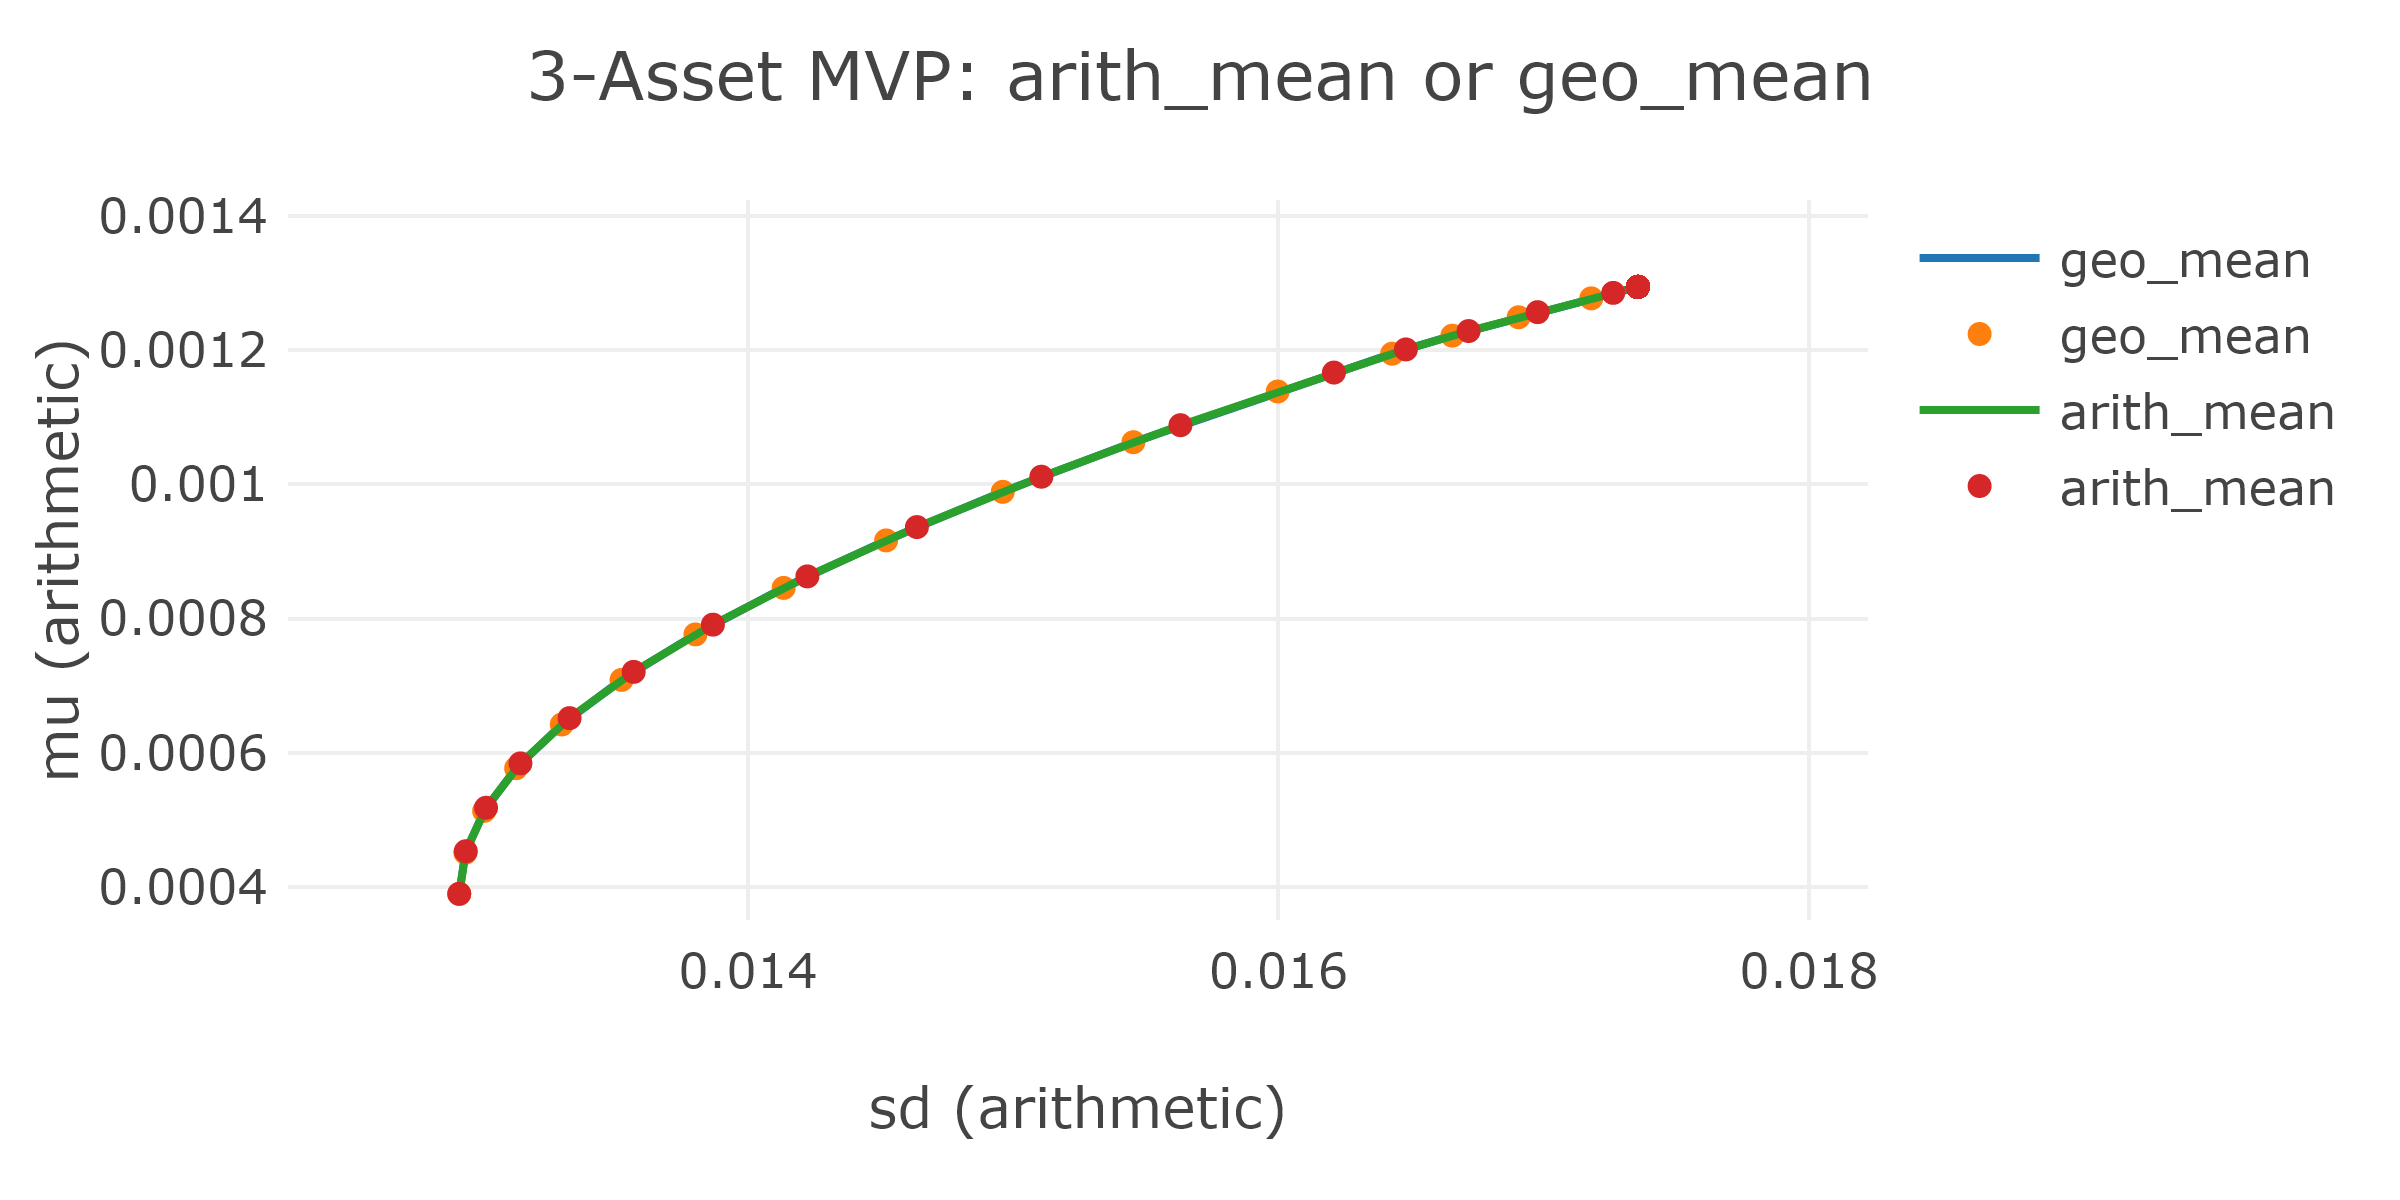
\includegraphics{gitbook-demo_files/figure-latex/unnamed-chunk-4-1.png}

\begin{Shaded}
\begin{Highlighting}[]
\CommentTok{\#\}}
\end{Highlighting}
\end{Shaded}

Now we can calculate the expected daily returns and the covariance matrix for the 3 assets:

\begin{Shaded}
\begin{Highlighting}[]
\NormalTok{mu }\OtherTok{\textless{}{-}} \FunctionTok{as.vector}\NormalTok{((}\FunctionTok{last}\NormalTok{(}\FunctionTok{ret\_to\_cumret}\NormalTok{(returns))}\SpecialCharTok{/}\DecValTok{100}\NormalTok{)}\SpecialCharTok{\^{}}\NormalTok{(}\DecValTok{1}\SpecialCharTok{/}\FunctionTok{nrow}\NormalTok{(returns))}\SpecialCharTok{{-}}\DecValTok{1}\NormalTok{)}
\NormalTok{mu}
\end{Highlighting}
\end{Shaded}

\begin{verbatim}
## [1]  0.00237647165  0.00106873765 -0.00004734503
\end{verbatim}

\begin{Shaded}
\begin{Highlighting}[]
\NormalTok{cov }\OtherTok{\textless{}{-}} \FunctionTok{as.matrix}\NormalTok{(}\FunctionTok{nearPD}\NormalTok{(}\FunctionTok{cov}\NormalTok{(returns))}\SpecialCharTok{$}\NormalTok{mat)}
\NormalTok{cov}
\end{Highlighting}
\end{Shaded}

\begin{verbatim}
##              AAPL         GOOG          IBM
## AAPL 0.0008635447 0.0005337733 0.0004356540
## GOOG 0.0005337733 0.0005827306 0.0004086774
## IBM  0.0004356540 0.0004086774 0.0006625236
\end{verbatim}

At this moment we have all the needed data to solve the MVP \eqref{eq:MVP} with \(\lambda \in \{0.01, 0.02, ..., 0.99, 1\}\). Afterwords we calculate the annual returns and standard deviation and draw the efficient frontier and the composition of the portfolios:

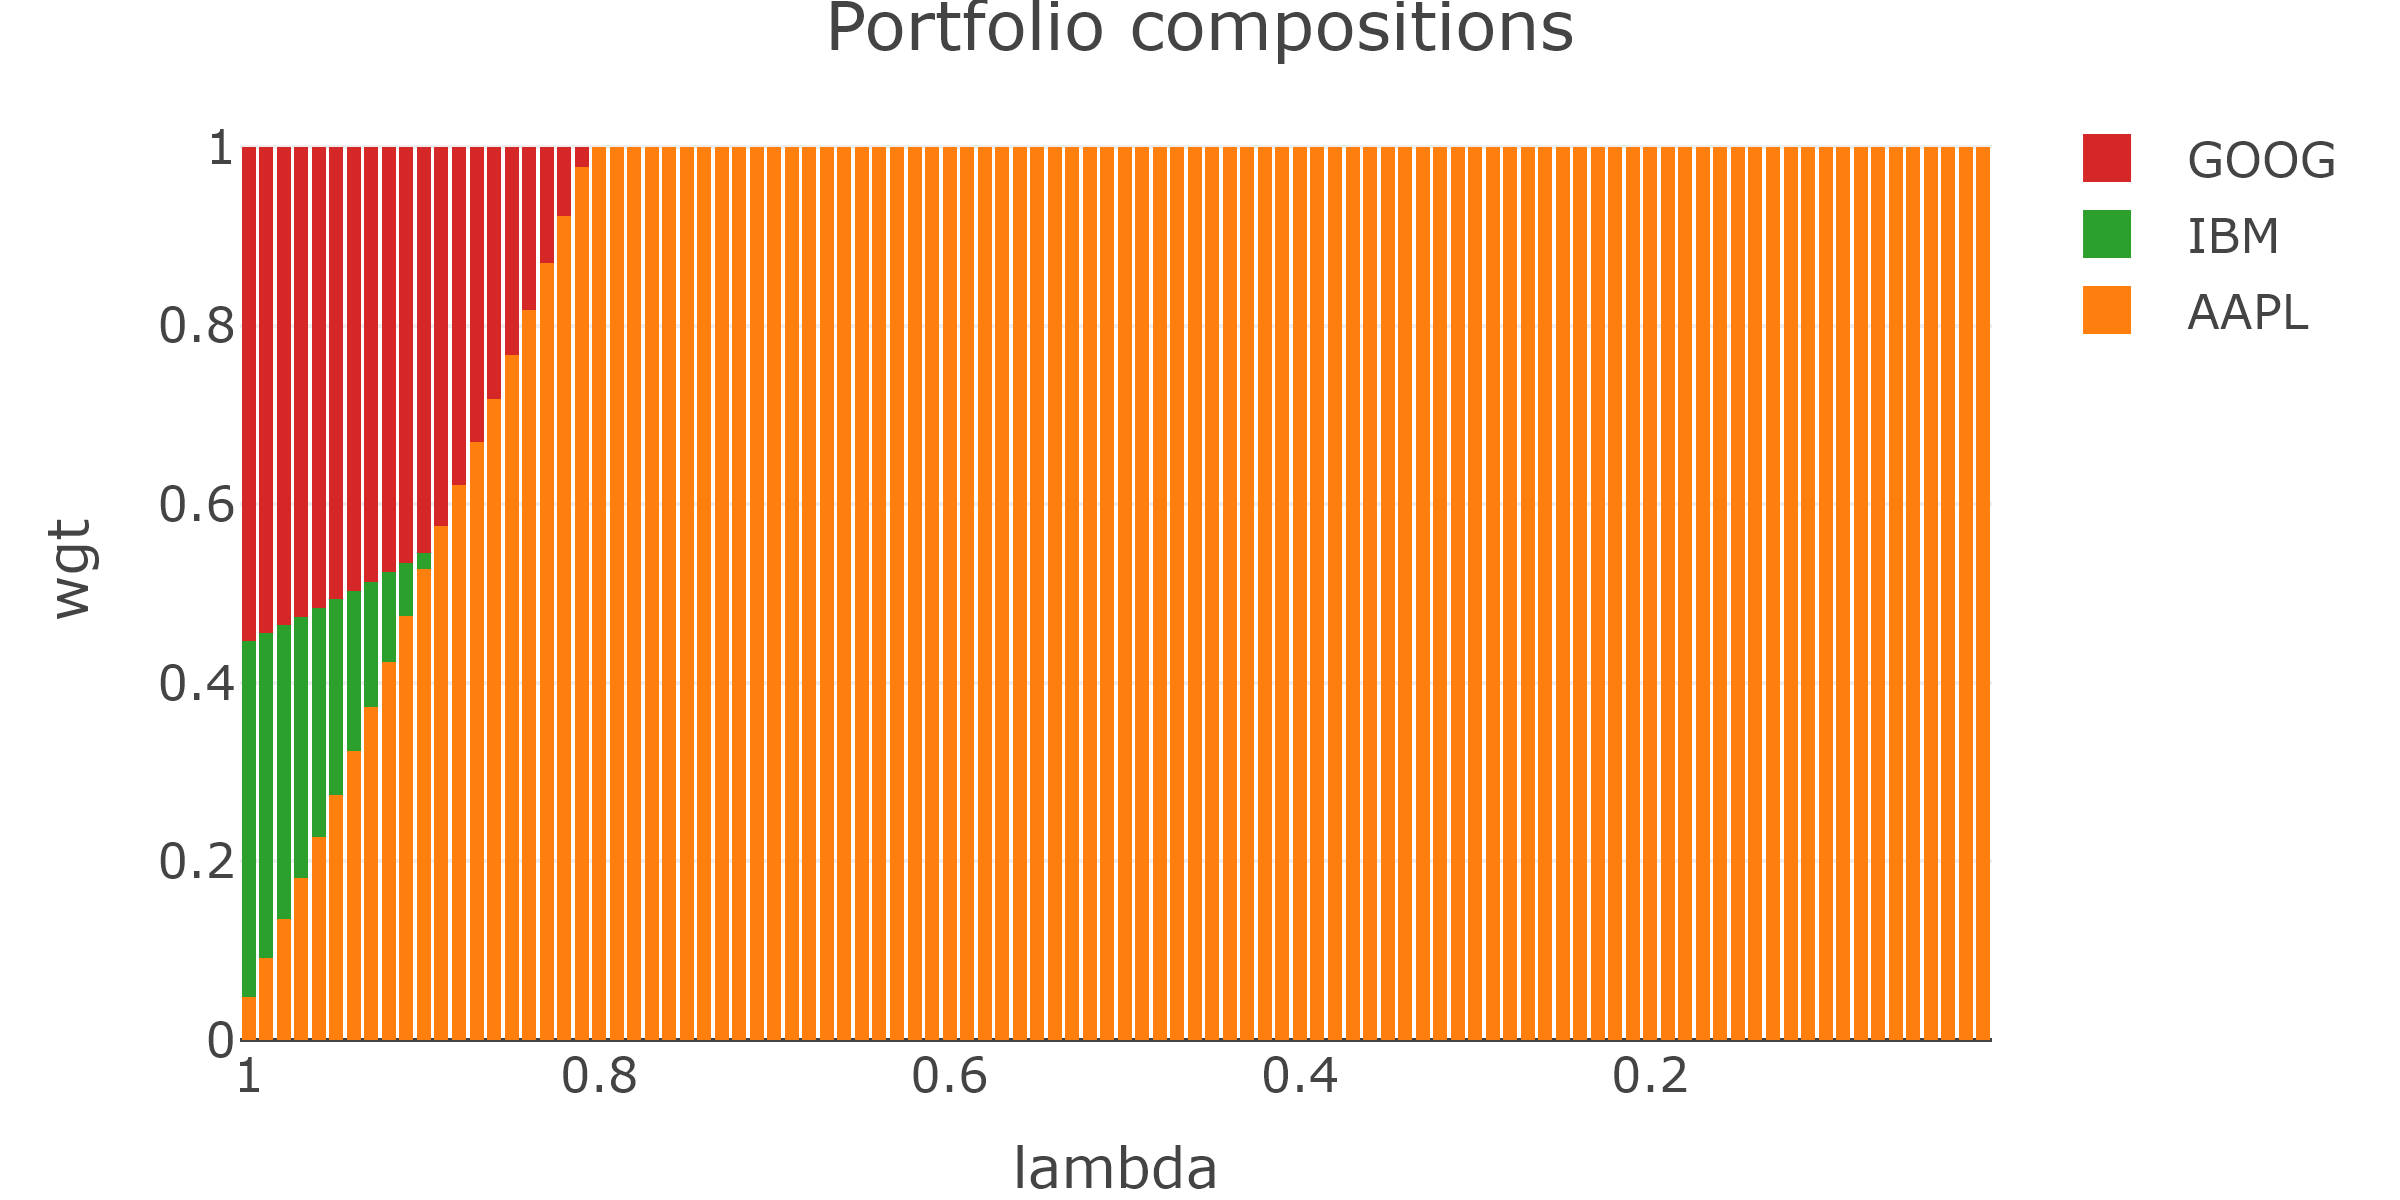
\includegraphics{gitbook-demo_files/figure-latex/unnamed-chunk-6-1.pdf} \includegraphics{gitbook-demo_files/figure-latex/unnamed-chunk-6-2.pdf}

\hypertarget{index-tracking-portfolio-itp}{%
\section{Index-tracking portfolio (ITP)}\label{index-tracking-portfolio-itp}}

Indices are baskets of assets which are used to track the performance of a specific group of assets. For example tracks the good known Standard and Poor's 500 index (short: S\&P 500) the largest 500 equitys in the United States. All indices are not investible and only serve for the visualisation of the performance of these groups of assets without transaction costs. Asset managements adopted these indices as benchmarks to compare there fund performances. Each fund has its own benchmark which contains roughly the same assets that could be purchased by the manager. If the fund under performs his benchmark, it could be a indicator for a bad decision from the fund manager. Thats why all fund managers are eager to beat there benchmarks with wisely choosen investments. The past has proven that this is rearly achived with activ managemnt after costs (quelle studie activ passiv). This is the reason why passiv managed funds with the goal to track there benchmarks are becoming more frequent. Exactly this can be archived with Index-tracking portfolios (ITP) which aim to replicate the performance of a benchmark. This can be done by either full-replication or sparse-replication. A full-replication, which produces the exact performance we aim for, isn't possible in most cases because not all assets of a index are investable. And if so it wouldnt be wise because benchmarks with multiple indices can contain more than ten thousand single assets which will produce a huge amount of transaction costs. The most common way to go is a sparse replication of the performance. To do so the portfolio manager has to define his benchmark which has a overlap with his investment universe of his fund. Afterwards he will reduce this universe by some rules of the investor, liqudity and availability. Now he can start to optimize a portfolio, including the investors constraint, to replicate the benchmark performance. Usually, this is done by reducing the difference between the daily returns of the ITP and the benchmark:

\[
 minimize \ \ Var(r_{p}-r_{bm})
\]
First we need to substitude \(r_{p}\) to get the portfolio weights \(w\) as follows:
\[
  r_{p} = R * w
\]
Afterwards we solve the Variance until it is displayed as a quadratic problem of \(w\):
\[
 Var(r_{p}-r_{bm}) = Var(R * w - r_{bm}) = Var(R * w) + Var(r_{bm}) - 2 \cdot Cov(R*w,r_{bm}) 
\]
Now we need to solve each of the 3 terms, startign with the simplest

\[
Var(r_{bm}) = \sigma_{bm}^2 = constant
\]

The variance of the portfolio can be solved by looking at the proof in {[}\url{http://www.math.kent.edu/~reichel/courses/monte.carlo/alt4.7d.pdf} (proof auch selber machen){]} at the linear combination of random variables section:
\[
Var(R * w) = w^T * Cov(R) * w
\]

And the last term can be solved in general as (\url{https://bookdown.org/compfinezbook/introcompfinr/Multivariate-Probability-Distributions-Using-Matrix-Algebra.html} 3.6.5):
\[
  Cov(A*a, b) = Cov(b, A*a) = Cov(b, A)^T * a
\]

\begin{Shaded}
\begin{Highlighting}[]
\CommentTok{\# A = matrix(c(1,4,2,4,6,3,8,4,4,10), ncol=2)}
\CommentTok{\# a = c(0.2, 0.8)}
\CommentTok{\# b = c(4,4,5,5,7)}
\CommentTok{\# }
\CommentTok{\# cov(A \%*\% a, b)}
\CommentTok{\# t(a) \%*\% cov(A, b)}
\CommentTok{\# t(cov(A, b)) \%*\% a \# das hier wird gebraucht}
\end{Highlighting}
\end{Shaded}

This results in the final formula of the ITP:

\begin{equation}
  \begin{split}
   Var(r_{p}-r_{bm}) & = Var(R \times w - r_{bm}) \\
   & = Var(R \times w) - 2 \cdot Cov(R \times w,r_{bm}) + Var(r_{bm})  \\
   & = w^T \times Cov(R) \times w - 2 \cdot Cov(r_{bm}, R)^T \times w + \sigma_{bm}^2
   \end{split}
   \label{eq:ITP}
\end{equation}

The minimization problem of the ITP in the general stricture which all optimizers need is:
\[
  min(\frac{1}{2} \cdot b^T \times D \times b -d^T \times b)
\]
Because it is a minimization we can ignore constant terms and stretching coefficients and still find the same minimum. This results in the general substitution of the ITP as follows:
\[
  D = Cov(R)
\]
and
\[
d = Cov(r_{bm}, R)
\]

Now we need to add some basic constraints like in the MVP, to sum up the weights to 1 and being long only.

\hypertarget{example-itp}{%
\subsection{Example ITP}\label{example-itp}}

We will show the results of tracking the S\&P 500 with a tracking portfolio that can only invest in IBM, Apple and Google without going into details:
222233333344445

\begin{verbatim}
##      AAPL      GOOG       IBM 
## 0.2597104 0.3308051 0.4094845
\end{verbatim}

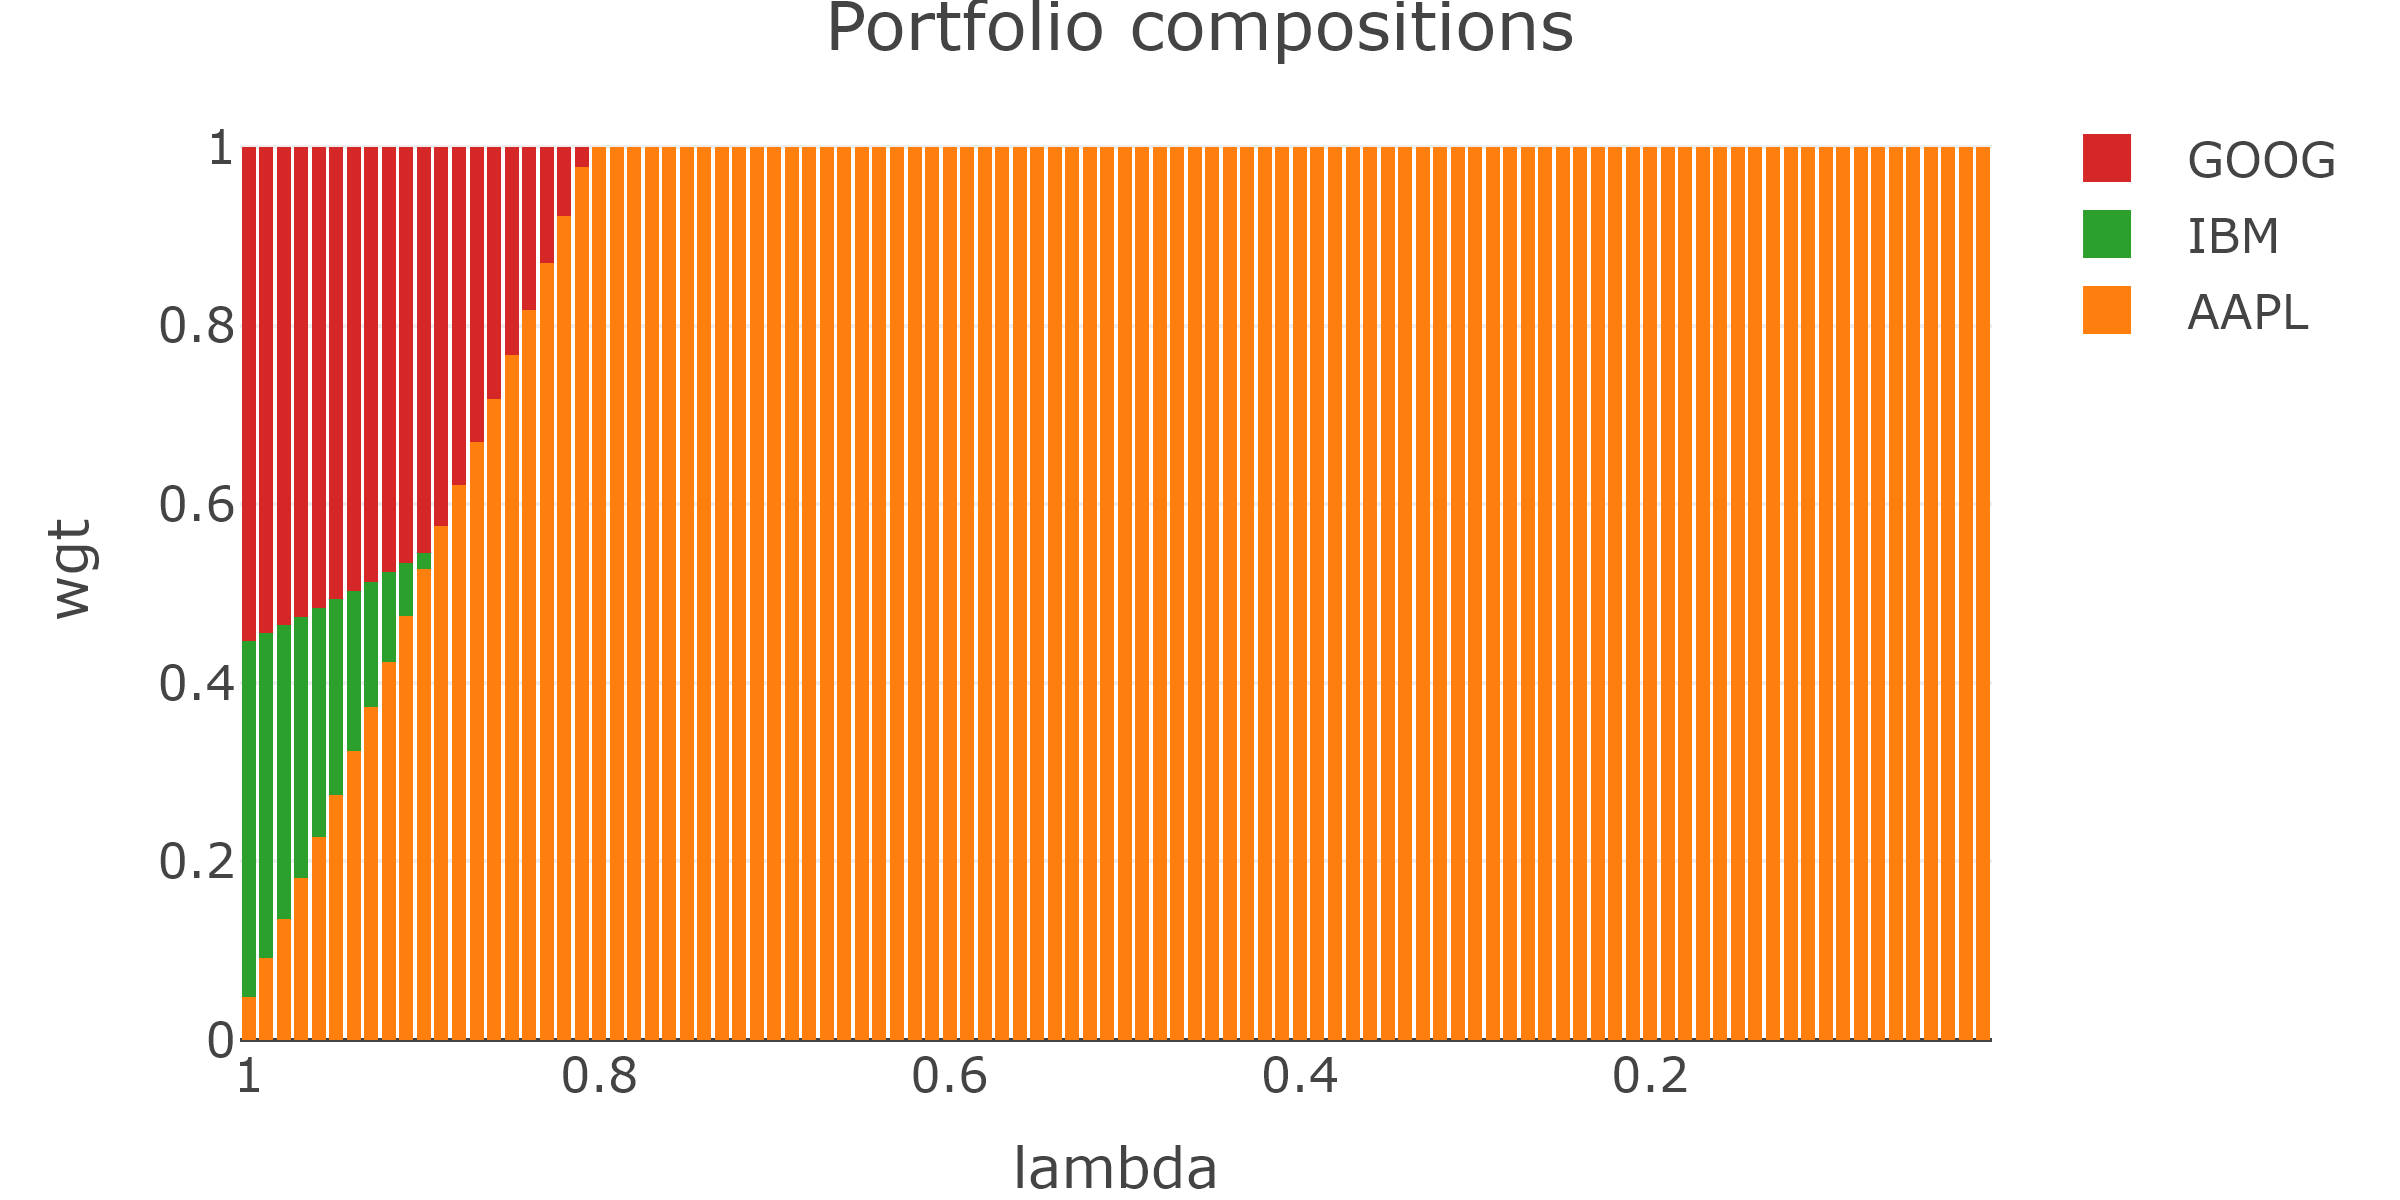
\includegraphics{gitbook-demo_files/figure-latex/unnamed-chunk-9-1.png}

\hypertarget{analytical_solver}{%
\chapter{Analytical\_Solver}\label{analytical_solver}}

example to solve problems with analytical solvers

\hypertarget{simple_particle_swarm_optimization}{%
\chapter{Simple\_Particle\_Swarm\_Optimization}\label{simple_particle_swarm_optimization}}

first pso examples and explainations

  \bibliography{book.bib,packages.bib}

\end{document}
